\documentclass[a4paper,11pt,article,twoside]{memoir}

%%%%%%%%%%%%%%%%
%%% PACKAGES %%%
%%%%%%%%%%%%%%%%

\usepackage{maplestd2e}	% Til maple input
\usepackage{multirow}  % Flere rows i tabeller
\usepackage{float}    % Pakke til at placere figurer hvor de fandme skal være!
\usepackage[english]{babel} 			    % Engelsk ordbog        			
\usepackage[utf8]{inputenc}					% Understøttelse af æ, ø og å Editor skal være sat op til UTF-8 encoding
\usepackage[T1]{fontenc}          			% Bruger en rigtig font til dansk output.
\usepackage{amssymb, amsmath}  				% Nice equations
\usepackage{listings}                       % Til at inkludere kode i teksten ved: \begin{lstlisting}
\usepackage{ulem}   			 
\usepackage{lscape}							% Pakke til at lave enkelte landscabe sider (\begin{landscape})
\usepackage{siunitx}						% Nice cmd til sienheder. Bl.a.: \num{.3e-4}
\usepackage{lmodern} 						% Fontpakke for pdflatex
\usepackage{wrapfig}						% Pakke til ordombrydning
\usepackage{subfig}			 				% Nice måde at samle flere figurer.
\usepackage[square,sort]{natbib}
		\bibpunct{[}{]}{;}{n}{,}{,}			% Citeringer til bøger mm. \citep
\usepackage[pdftex]{hyperref}				% Til flotte links
\usepackage{graphicx}						% Diverse billed sjov
\usepackage{mathrsfs}
\usepackage{amssymb}						% Math font
\usepackage[danish=quotes]{csquotes}		% Benytte for at kunne lave " tegnet
\usepackage[table]{xcolor}					% Farvekoder til tabeller
\usepackage{titlesec}
\usepackage{rotating}

\usepackage{geometry}						% Pakke til at ændre margen på enkelte sider

\usepackage{tikz}							%Tikz til at tegne flow chart 
\usetikzlibrary{shapes,arrows,chains}		%Tikz-library til figurer i flowchart
\usetikzlibrary{positioning}				%Positioning of boxes in flow chart
\titleformat{\section}{\normalsize\bfseries}{\thesection}{1em}{}
\captionsetup{margin=25pt,font={footnotesize,sf},format=hang}

%%%%%%%%%%%%%%%%%
%%% PAGESETUP %%%
%%%%%%%%%%%%%%%%%
 
\chapterstyle{article}						% Article layout
\def\thesection{\thechapter.\arabic{section}}% 1.1. Ønskes 1.A, ændr arabic til Alph
\settrimmedsize{297mm}{210mm}{*}			% Tilpasser Layout til a4
\setlength{\trimtop}{0pt}							
\setlength{\trimedge}{\stockwidth}				
\addtolength{\trimedge}{-\paperwidth}				
\settypeblocksize{634pt}{448.13pt}{*}				
\setulmargins{5cm}{*}{*}										
\setlrmargins{*}{*}{0.6}									
\setmarginnotes{17pt}{51pt}{\onelineskip}			
\setheadfoot{\onelineskip}{2\onelineskip}		
\setheaderspaces{*}{2\onelineskip}{*}
\checkandfixthelayout
\setlength{\parindent}{0 pt}
\makepagestyle{rapport}						% Laver en ny type sidehoved
\aliaspagestyle{chapter}{rapport}			% Sætter 'chapter'-sidehoved = 'ah'-sidehoved
\addtolength{\voffset}{-0.5cm}
\setlength{\headsep}{10 pt}
\hyphenation{spej-let mel-lem temperatur-udviklinger}                     	 	
% Hvis ord bliver delt forkert, kan de indskrives med den rigtige orddeling her.

%%%%%%%%%%%%%%%%%%
%% STYLE SETUP %%%
%%%%%%%%%%%%%%%%%% 

\pagestyle{rapport}							% Sætter 'rapport' til standard-sidehoved
\renewcommand{\chaptermark}[1]{         	% Opretter kommando til kapitelnavne i header
\markboth{\chaptername\ \thechapter.\ #1}{}}%Header og footer setup
\makeevenhead{rapport}{\leftmark}{}{\theauthor}
\makeoddhead{rapport}{\theauthor}{}{\titel}	
\makeheadrule{rapport}{\textwidth}{1pt}		
\makeoddfoot{rapport}{}{}{\thepage}			
\makeevenfoot{rapport}{\thepage}{}{} 

%%%%%%%%%%%%%%%%%%%%%%%%%%
%%%   PDF/EPS script   %%%
%%%%%%%%%%%%%%%%%%%%%%%%%%

\usepackage{epstopdf}						% Pakke der konverterer EPS til PDF

%%%%%%%%%%%%%%%%%%%%%%%
%%% CUSTOM COMMANDS %%%
%%%%%%%%%%%%%%%%%%%%%%%

%%%%%%%%% INCLUDEGRAPHICS %%%%%%%%%
%\graphicspath{{./figures/}}
%\newcommand{\placefigwof}[3]{						
%	\begin{figure}[htb!]
%		\begin{center}
%			\includegraphics[width=  #1\textwidth]{#2}
%		\end{center} 
%		\caption{#3} \label{fig:#2}
%	\end{figure}\\}
%
%\newcommand{\placefig}[4]{										
%	\begin{figure}[htb!]
%		\begin{center}
%			\includegraphics[width=  #1\textwidth]{#2}
%			\footnotemark
%		\end{center} 
%		\caption{#3} \label{fig:#2}
%	\end{figure}\\
%	\footnotetext{#4}}
%	
%\newcommand{\placefigswof}[4]{								
%	\begin{figure}[!htb]
%		\begin{center}
%    		\subfloat{\includegraphics[width=  #1\textwidth]{#2}}\;
%    		\subfloat{\includegraphics[width = #1\textwidth]{#3}}
%    		\footnotemark
%			\caption{#4} \label{fig:#2,#3}
%		\end{center}	
%	\end{figure}\\}	
%	
%\newcommand{\placefigs}[5]{	
%	\begin{figure}[!htb]
%		\begin{center}
%    		\subfloat{\includegraphics[width=  #1\textwidth]{#2}}\;
%    		\subfloat{\includegraphics[width = #1\textwidth]{#3}}
%    		\footnotemark
%			\caption{#4} \label{fig:#2,#3}%\ref{fig:#2,#3}
%		\end{center}	
%	\end{figure}\\
%	\footnotetext{#5}}
	
%%%%%%%%% EASY-MATH  %%%%%%%%%
\newcommand{\mb}[1]{\mathbf{#1}}
\newcommand{\vek}[1]{{\mathbf{\bar{#1}}}}
\newcommand{\maple}[1]{\textcolor[rgb]{1,0,0}{\\> $\mathtt{#1}$;}}
\newcommand{\mapleo}[1]{\textcolor[rgb]{0,0,1}{\begin{displaymath} \mathtt{#1}\end{displaymath} }}

%%%%%%%%% BLANDET  %%%%%%%%%
\newcommand{\dul}[1]{\underline{\underline{#1}}}% Dobbelt understregning

%%%%%%%%%%%%%%%%%%%%
%%% AUTHOR SETUP %%%
%%%%%%%%%%%%%%%%%%%%

\author{Mads Bornebusch, Tobias Tuxen og Kristian Lauszus}															%Forfatter
\newcommand{\titel}{30010 Programmeringsprojekt}   					%Titel
\newcommand{\subtitle}{Reflex Ball \\Gruppe Nummer: 15}	%Undertitel
\newcommand{\dato}{\today}												%Dato \today kan bruges for at indsætte compile dato.

%%%%%%%%%%%%%%%
%%% RAPPORT %%%
%%%%%%%%%%%%%%%

\begin{document}

	%%% FORSIDE %%%
	\frontmatter
	\thispagestyle{empty}
	\begin{center}
\vspace*{\stretch{1}}
% rule laver en linje på tværs af siden
\rule{\textwidth}{1mm}\\
\vspace{1cm}
% Her vælger en kæmpe skrifttype og fed skrift
\Huge\bfseries \titel\\
\vspace{0.7cm}
\rule{\textwidth}{1mm}\\

\begin{figure}[h!]
	\centering
	\begin{minipage}{0.40\linewidth}
	\begin{center}
	\includegraphics[scale=0.55]{figs/mads.jpeg} \\
	Mads Friis Bornebusch (s123627)\\ [10pt]
		\vspace{0.15cm}
	\end{center}
	\end{minipage}
\end{figure}

\begin{figure}[h!]
	\centering
	\begin{minipage}{0.40\linewidth}
	\begin{center}
	\includegraphics[scale=0.55]{figs/tobias.png} \\
	Tobias Tuxen (s120213)\\[10pt]
		\vspace{0.15cm}
	\end{center}
	\end{minipage}
\end{figure}

\begin{figure}[h!]
	\centering
	\begin{minipage}{0.40\linewidth}
	\begin{center}
	\includegraphics[scale=0.55]{figs/kristian.jpeg} \\
    Kristian Sloth Lauszus (s123808) \\ [10pt]
		\vspace{0.15cm}
	\end{center}
	\end{minipage}
\end{figure}


\vspace*{\stretch{2}}
\end{center}
\begin{flushleft}
\subtitle\\
DTU Space\\
\dato
\end{flushleft}


	
	%%% INDHOLDSFORTEGNELSE OG ABSTRACT %%%
		\chapter{Abstract}

In this programming project we have written and designed all the code to the game Reflex Ball. The code has been written in C in the compiler Z8Encore! and has been implemented on a Zilog 6403 Mircrocontroller. \\ \\
We have concluded that the written code implements the desired circuit on the Microcontroller as as all the different facilities of the game has been thoroughly tested and is in compliance with the expected result. In the end we have a fully functional Reflex Ball Game with many expansions, which amongst others, include bricks (Arkanoid style), power-ups, different levels and steering-wheel game controller. So far no bugs has been found in the final version of the game.

\begin{figure}[h!]
\centering
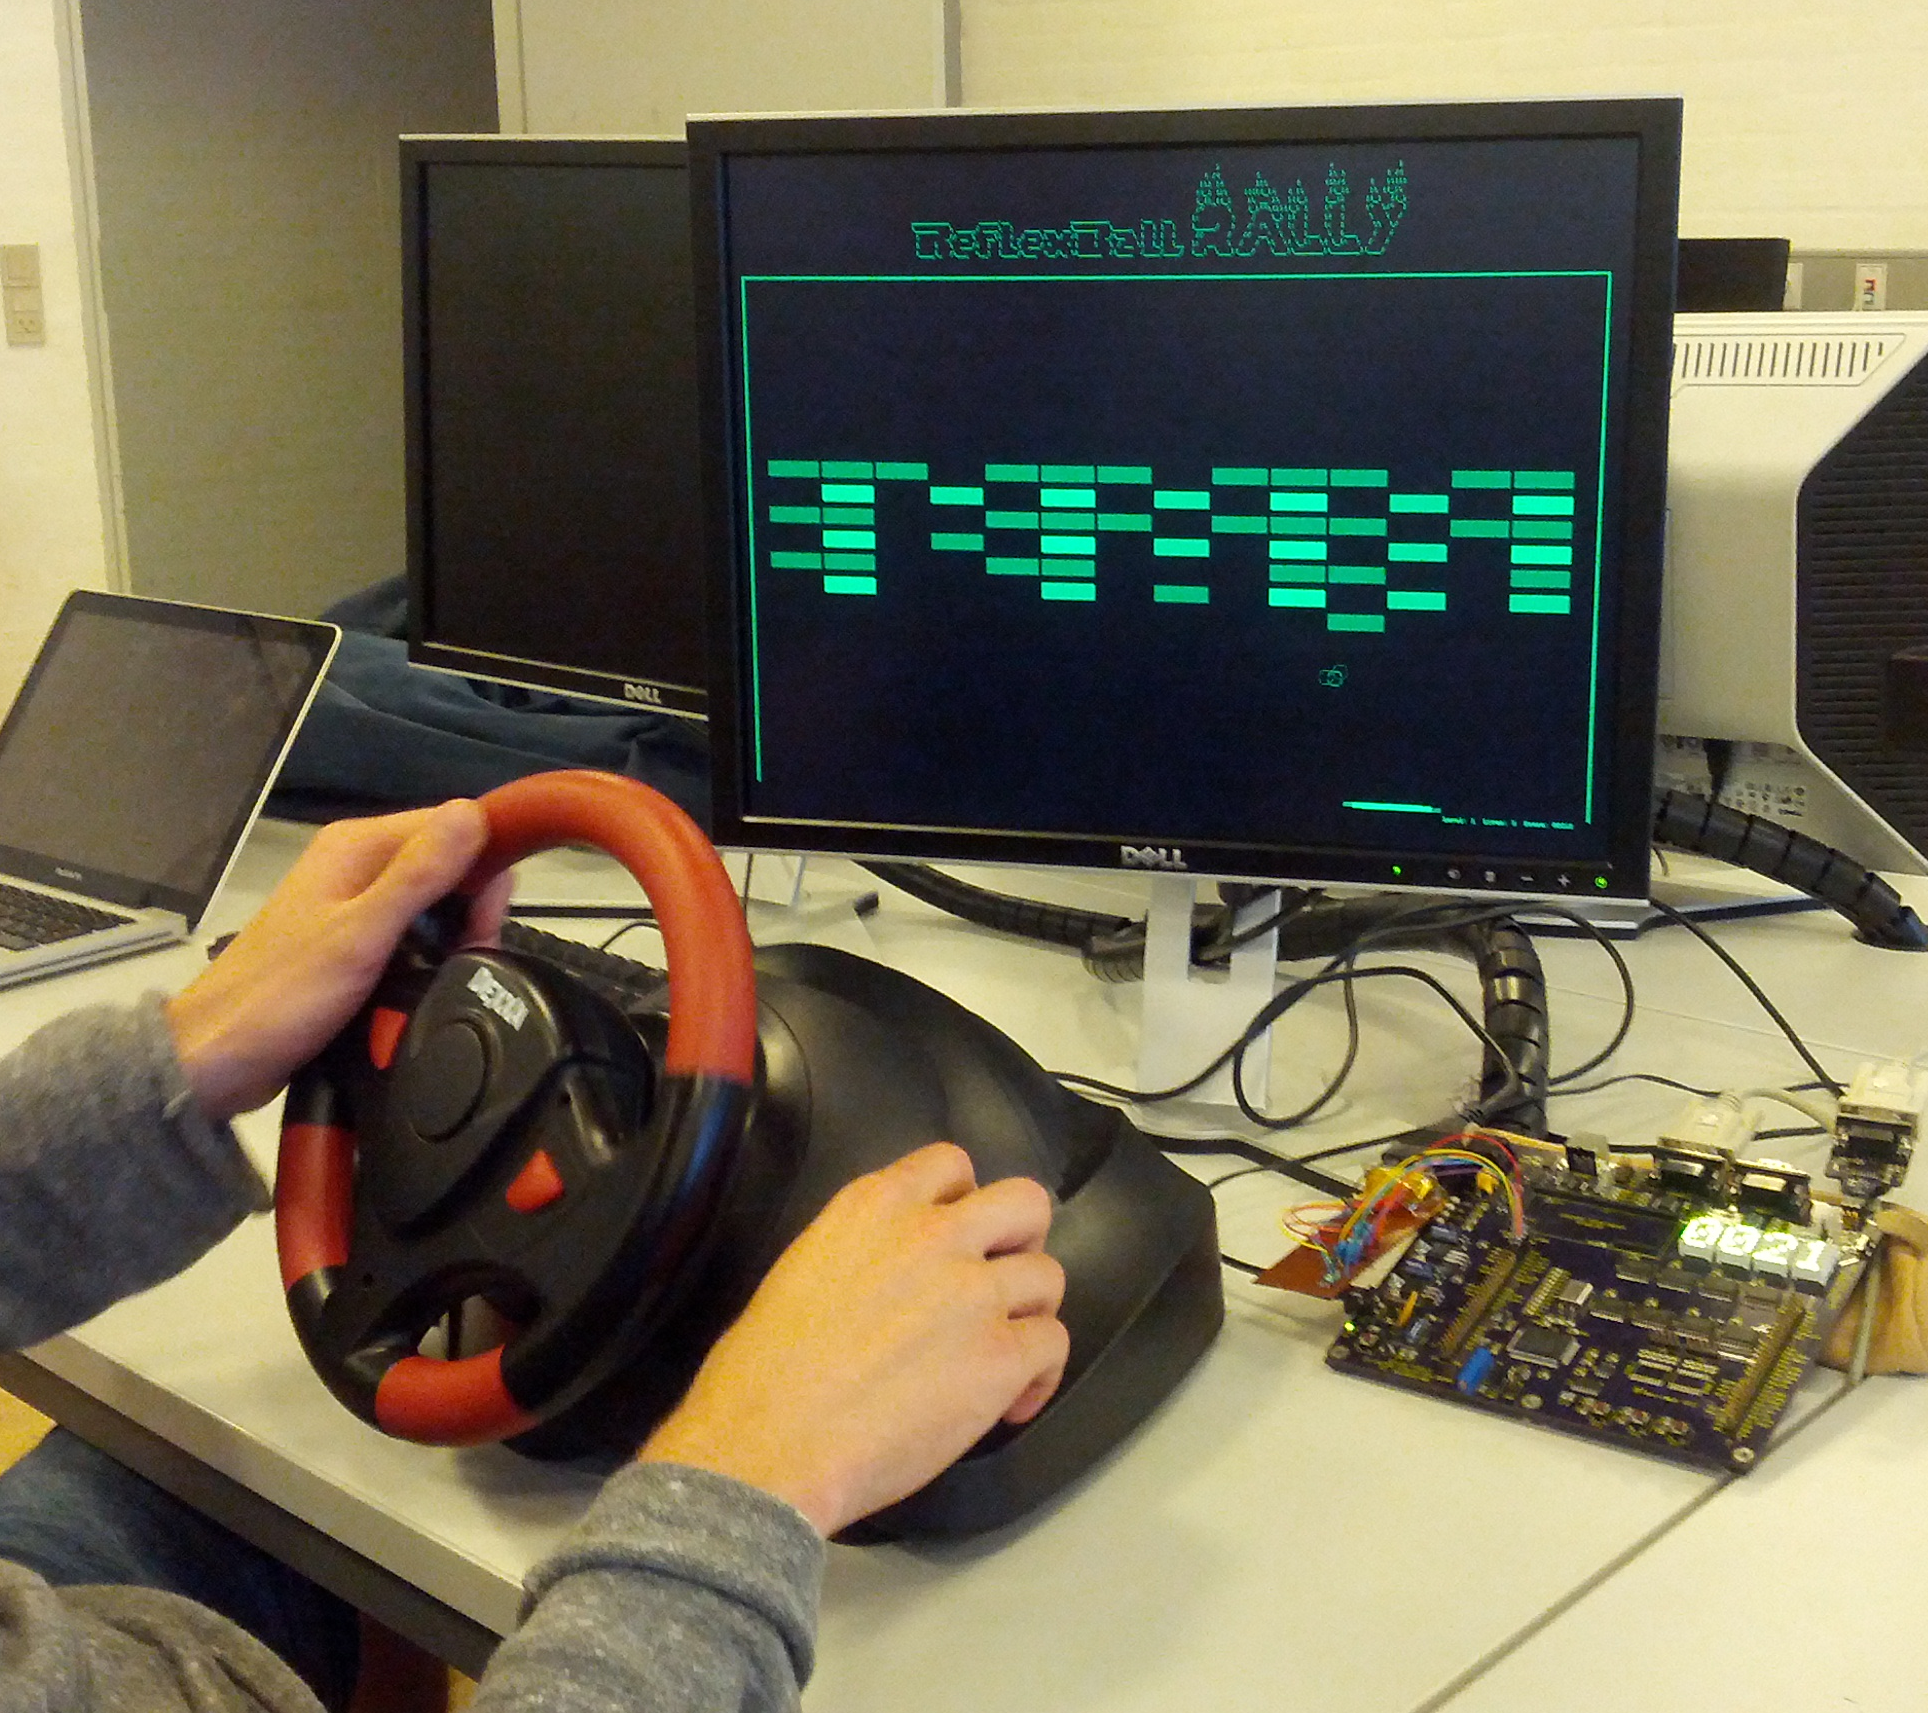
\includegraphics[scale=0.5]{figs/forside.png}
\caption{Screenshot from our implementation of ReflexBall}
\label{fig:awesome}
\end{figure}
		\chapter{Resumé}

I dette programmeringsprojekt har vi skrevet og designet al koden til spillet Reflex Ball. Koden er skrevet i C i compileren Z8Encore! og implementeret på en Zilog 6403 mircocontroller. \\ \\
Vi har konkluderet at den skrevne kode implementerer det ønskede kredsløb på Mircrocontrolleren, da alle spillets facetter er blevet gennemtestet og giver det ønskede output. Som slutresultat har vi et fuldt funktionelt ReflexBall-spil med mange udvidelser der bl.a. inkluderer forskellige typer brikker (Arkanoid-stil), sværhedsgrader, forskellige levels og styring med ret. Der er indtil videre ikke fundet nogle bugs i slutversionen af spillet.\\ \\
		\newpage
		\chapter{Forord}

Denne rapport er skrevet som en del af eksaminationen i DTU kursus 30010 - Programmeringsprojekt. Alle tre, på forsiden nævnte, gruppemedlemmer har bidraget til rapporten på lige vis. Vi har lavet alle forberedelsesøvelser, skrevet koden og afsnittene i rapporten i fællesskab. Denne rapport beskriver vores arbejde og resultater.
\\

Vi har valgt kommenterer hele koden på engelsk i det vi har gjort den tilgængelig Open Source på følgende side: \url{https://github.com/Lauszus/ReflexBall}.\\
Derudover kan dokumentation af source koden findes på siden: \url{http://lauszus.github.io/ReflexBall/}.
\\

\begin{figure}[h!]
\centering
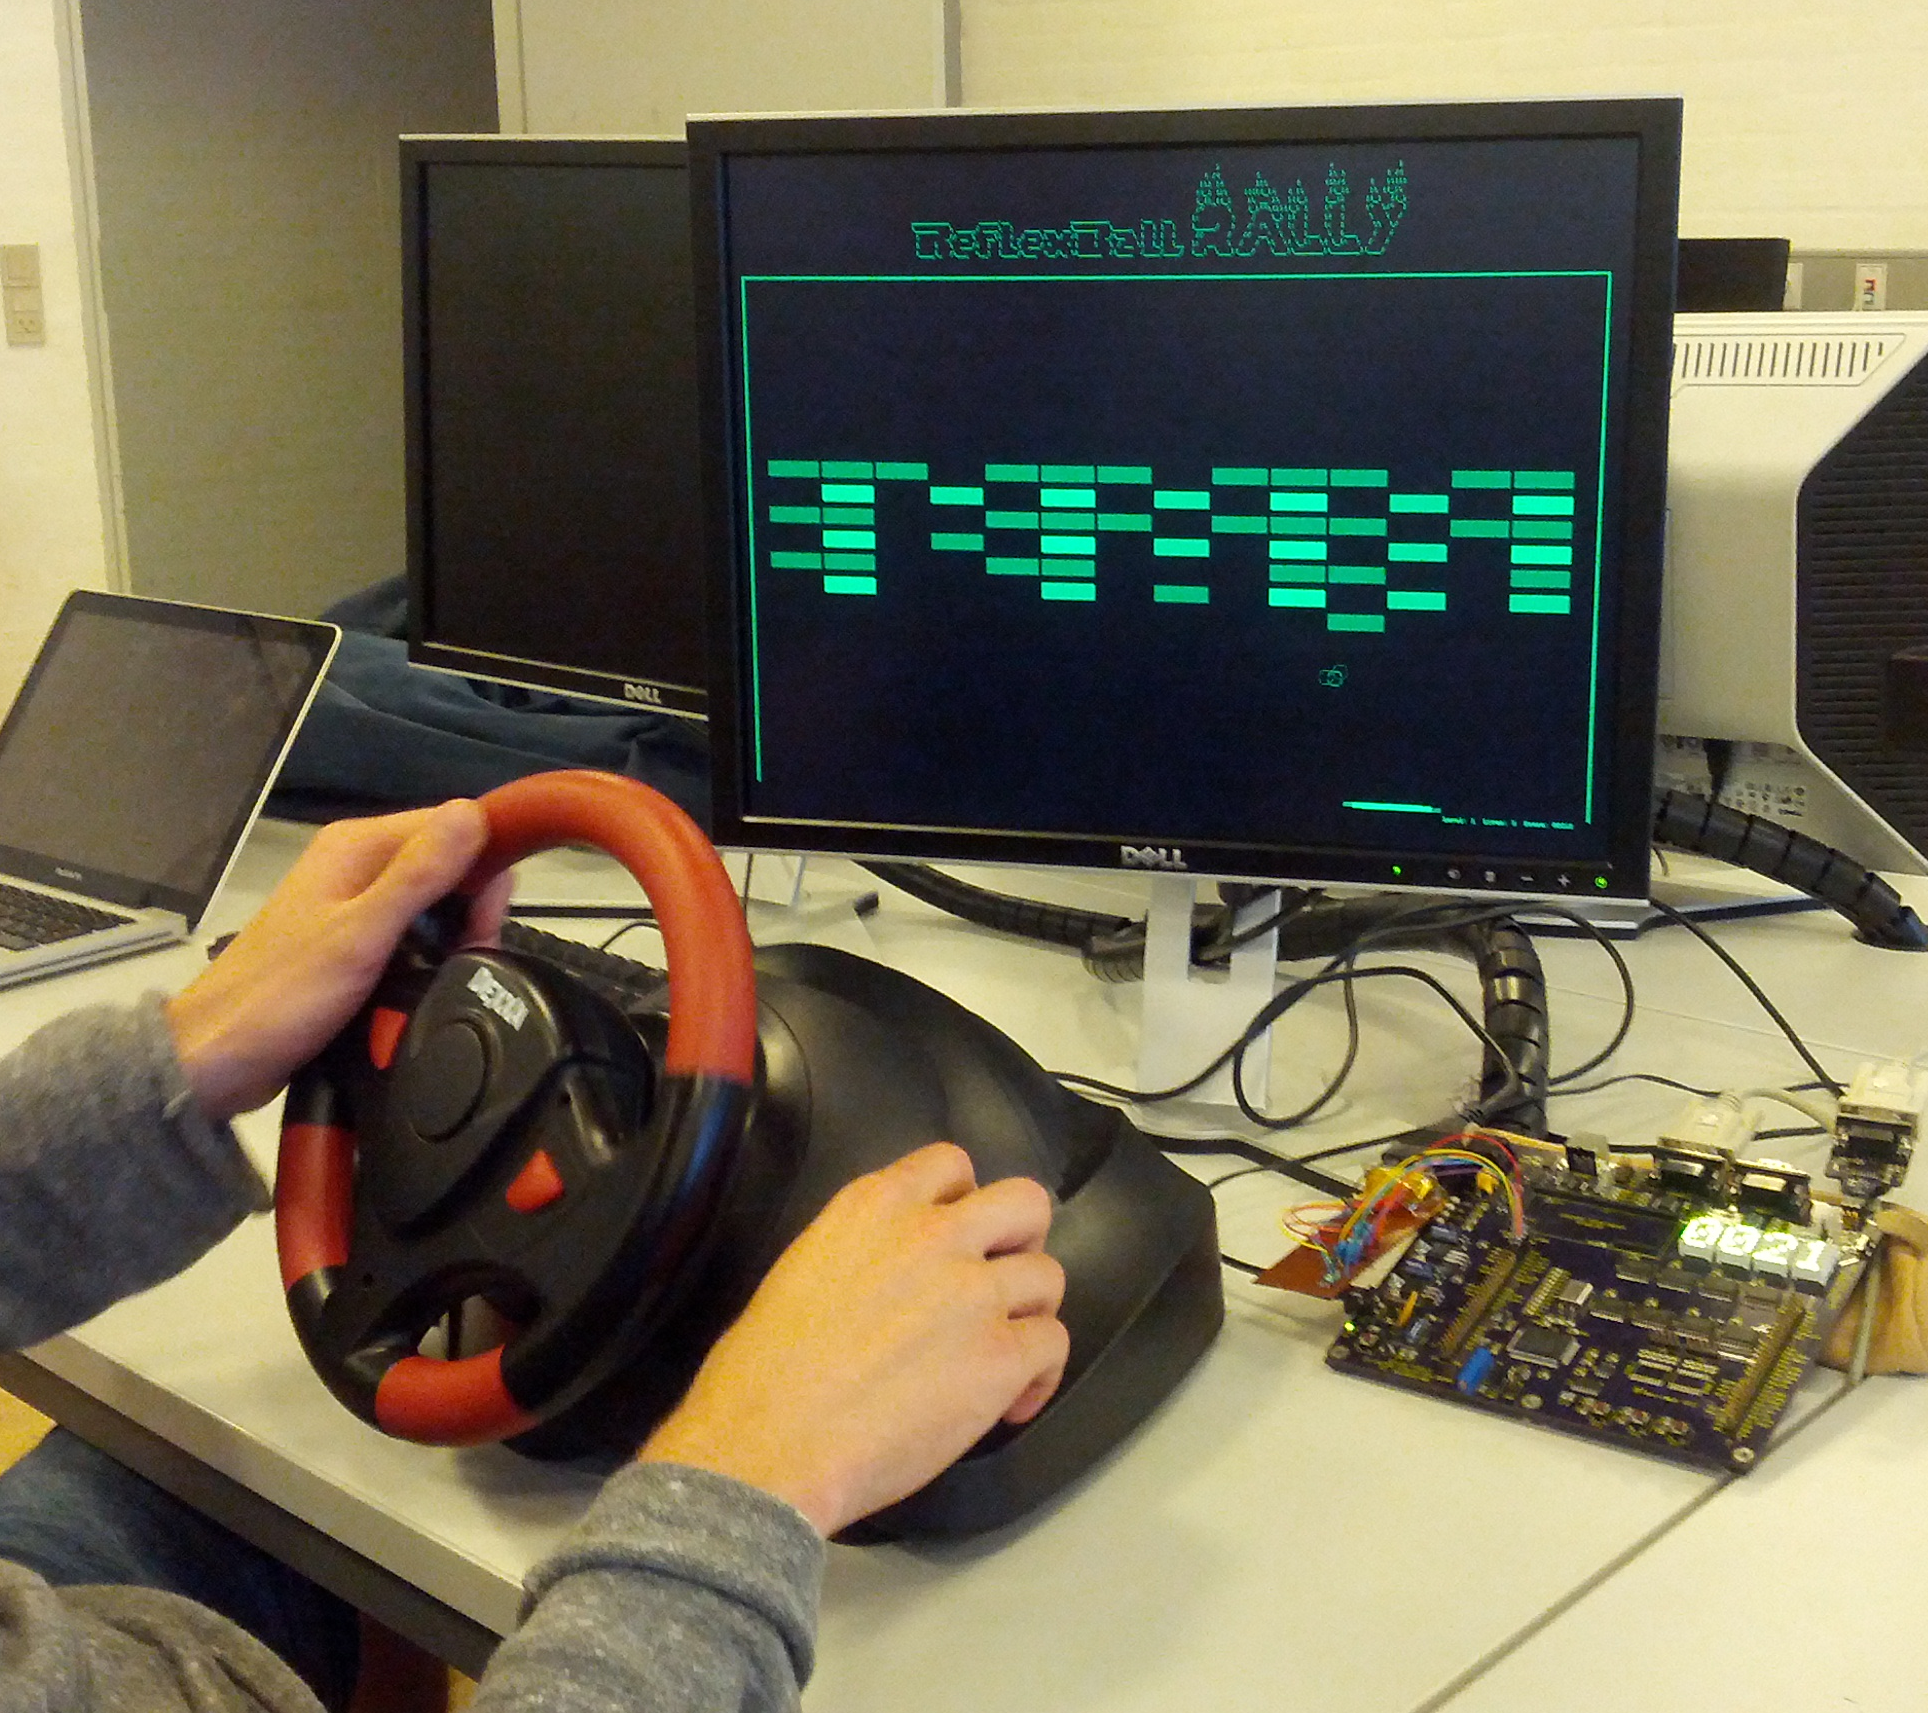
\includegraphics[scale=0.17]{figs/forside.jpg}
\caption{Et igangværende spil ReflexBall RALLY}
\label{fig:forside}
\end{figure}
		\newpage
		\tableofcontents*						% Indholdsfortegnelse (fjern * hvis der skal stå "Indhold")
%        \listoffigures*						% Figurliste

		
	%%% RAPPORTINDHOLD %%%
		\mainmatter
%		\input{tex/maple}
		\chapter{Introduktion}

This report documents the design and implementation of the control part of a vending-machine for soft-drinks. \\

The project was divided into three laboratory exercises, in which parts of the system was designed. After the finalization of all three laboratory exercises a complete vending machine control circuit was designed and implemented on a Basys2 FPGA board. The optional parts of the lab exercises is included in the elaboration of each of the exercises, which also redefines some of the mandatory functions, and update/change them as the requirements of each part changes a we move towards the finished control part. \\
		\chapter{Specifikationer}

Nedenfor er vores forskellige delmål i projektet. Spillet skal have de nedenstående funktionaliteter. Listen kan derfor ses som kravene til hvad vores spil skal kunne og er samtidig opdelt på en logisk måde så man kan starte fra toppen af og arbejde sig igennem delmålene indtil man har et færdigt spil der fungerer og ser ud efter vores hensigt. Delmålene er samtidig bygget op på en sådan måde, at skulle der ikke være tid til at nå det hele, har man stadigvæk et fuldt funktionelt spil. Det vil altså sige at vi arbejder fra basale funktionaliteter ud mod mere specifikke og detaljerede elementer.\\

\textbf{Delmål Basics}
\begin{itemize}
\item Detektere tastatur-input så keyboardet kan bruges til at styre striker
\item Tegne banen
\item Bevæge strikeren
\item Bevægelig bold
\item Bolden reflekteres af striker, loft og vægge
\item Det skal detekteres når bolden er under strikeren (man er død)
\end{itemize}

\textbf{Delmål advanced}
\begin{itemize}
\item Liv-system, så man har 3 liv inden man bliver Game Over
\item Pointsystem
\item Ændring i boldhastighed som ens score stiger
\item Internt 18.14 koordinatsystem, så boldens bevægelse kan laves som en enhedsvektor der kan roteres rundt
\item Bolden skal starte i en tilfældig vinkel
\item Striker-zoner, så boldens afbøjningsvinkel afhænger af hvor den rammes 
\item Stor bold, der fylder 4x2 monospace-karakterer.
\item {Forskellige sværhedsgrader}
\item {Brikker og forskellige baner}
\end{itemize}
	

\textbf{Brikker}
\begin{itemize}
\item Banen skal indeholde brikker
\item Der skal være forskellige typer af brikker (forskellig antal liv)
\item Der skal være forskellige levels med brikker i forskellige mønstre
\item Når bolden rammer brikker og kanter skal den reflekteres på en logisk måde så fysikken i spillet ser realistisk ud
\end{itemize}

\textbf{Helhedsindtryk}
\begin{itemize}
\item LED display med score, liv og levels
\item Menu hvor man kan vælge sværhedsgrad
\item Beskeder ved Game Over
\item Besked hvis spillet vindes
\item Implementering af ASCII-Art tekst og billeder til Menu, Game Over og Win
\end{itemize}

\textbf{Hardware}
\begin{itemize}
\item Styring med intern hardware (knapper på microcontrolleren)
\item Tilslutning af ekstern hardware (DEXXA Steering Wheel)
\end{itemize}

Vi har lagt en del vægt på at spillet skal se realistisk ud og at bolden, strikeren og brikkerne skal flytte sig på en realistisk måde. Vi vil forsøge at lave spillets fysik så dette er opfyldt, så bolden bevæger sig så naturligt og logisk som muligt. 

		\chapter{Struktur}
\section{Basics}
Da vi skulle planlægge projektet valgte vi efter en brainstorm at dele projektet op i en mængde delmål vi ville have implementeret. Delmålene i kategorien basics var dem vi skulle implementere for at have et fungerende spil. Vi fandt frem til at det ville være følgende funktionaliteter:
\begin{itemize}
\item \textbf{Keyboard input}
\item \textbf{Bevægelig bold og striker (med clear)}
\item \textbf{Reflex-logik på kanter og hjørner}
\item \textbf{Game start og game over}
\end{itemize}
Vi vil i det følgende forklare hvordan disse delmål blev implementeret. 

Hvordan implementerede vi keyboardinput?
\texttt{kode tekst tekst}

\subsection{Keyboard input}


\section{Advanced}
Efter alle basics var færdigimplementeret, havde vi planlagt at lave nogle mindre udvidelser til spillet. Disse omfatter dels implemention af liv og pointsystem, men også videreudviklinger af basic-funktionaliteterne, sådan så deres bagvedliggende virkemåde gøres mere avanceret. Advanced inkulderer følgende.

\begin{itemize}
\item \textbf{Liv}. Som i ethvert andet arkade-spil har vi implementeret liv, sådan så man starter med tre og bliver Game Over, når der er nul liv tilbage.

\item \textbf{Score}. Point-systemet er opbygget sådan så det giver 1 point hver gang man rammer en brik og et ekstra point når brikken dør (går fra 1 til 0 liv). Det giver ingen point når bolden rammer strikeren, hvilket skyldes at man ikke skal have credit for tålmodighed.

\item \textbf{Hastighed}. Hastigheden hvormed bolden bevæger sig afhænger dels af hvor mange point man har, dels af hvilken sværhedsgrad man spiller på. På easy bliver boldens hastighed sat op for hver 10. point man får, på medium for hver 5. point man får, på hard for hver 2. point man får og på Chuck Norris, tja hvem ved?

\item \textbf{Vilkårlig startvinkel}. Når bolden skydes af bliver den sendt afsted i en vilkårlig vinkel på mellem 45 og 135 grader. Det vil sige lodret op fra strikeren plus minus op til 45 grader. Dette er implementeret for at man ikke kan time startvinklen så man er sikker på den altid rammer et bestemt sted.

\item \textbf{Striker-zoner}. Strikeren er opbygget sådan så den altid skal bestå af et lige antal felter. Dens midterste venstre felt har en afbøjningsvinkel på indgangsvinkel plus 0 grader, og dens yderste venstre felt har en afbøjningsvinkel på indgangsvinkel plus 45 grader. Hvert felt mellem det midterste venstre til det yderste venstre felt, har så en stigende afbøjningsvinkel, hvor den vinkel der bliver lagt til hvert felt er 45 grader divideret med antallet af felter fra det midterstre venstre (eksklusiv) til det yderstre venstre (eksklusiv). Højre-siden af strikeren fungerer på præcis samme måde, bare med omvendt fortegn, sådan så afbøjningsvinklen på midterste højre felt er lig indgangsvinklen og afbøjningsvinklen på yderstre højre felt er lig indgangsvinklen minus 45 grader.\\

Strikeren er lavet på denne måde så dens bredde er meget fleksibel. Fx bruges der forskellige Striker-størrelser på spillets forskellige sværhedsgrader og dette er så bare implementeret ved at ændre på størrelsen af \texttt{striker.width}. Så sørger spillet selv for at inddele Striker-zonerne. 

\item \textbf{Internt 18.14 koordinat-system}. I basic-implementationen af spillet satte vi bolden til at rykke sig et bestem antal monospaces hver gang den bevægede sig. Men med denne implementation er hele banens indre struktur blevet gentænkt sådan så bolden bevæger sig som en vektor i et koordinatsystem. Vi har lavet en \texttt{Ball struct} sådan så bolden hele tiden kender sine egne (x,y)-koordinater, samt dens egen enhedsvektor (altså retning hvori den bevæger sig). Når bolden bevæger sig sker der det at dens vektors (x,y)-koordinat lægges til boldens (x,y)-koordinat. Derefter tjekkes om bolden er død eller har ramt en brik, en væg, et hjørne, strikeren eller loftet. Hvis intet af dette er tilfældet, slettes boldens gamle koordinater ved at der på disse felter tegnes blanke mellemrum. Derefter afrundes boldens (x,y)-koordinater til nærmeste heltal ved at kigge på 1. bit efter kommaet, det vil sige boldens x- hhv. y-koordinats 19. bit (Da det tænkte komma er sat mellem 18. og 19. bit). Hvis denne er 0 rundes ned og ellers rundes op. Nu kendes boldens (x,y)-koordinat i heltal og den kan derfor indtegnes på banen.\\


\item \textbf{bolden bevæger sig med samme hastighed i både x- og y-retning}. Vi havde et problem med at det på skærmen lignede at boldens hastighed variede meget afhængigt af om dens vektor var relativt vandret (lille absolut y-komposant) eller relativt lodret (lille x-komposant). Dette skyldes at monospace-karakteren er meget tæt på at være dobbelt så høj som den er bred. Vores løsningen på dette var at gøre boldens vektors x-komposant dobbelt så stor, ved at bitshifte den en til venstre. På den måde bevæger bolden sig i virkeligheden aldrig som en enhedsvektor, da det er ekstremt usandsynligt at boldens vektors x-komposant skulle blive nul.

\item Stor bold. Vi har lavet en \texttt{Ball struct} der ud en bredde, højde i form af et

\item \textbf{Putty Terminal}. Som en del af de avancerede mål, skiftede vi fra Hyper Terminal over til Putty Terminal. Den eneste grund til dette er man i Putty Terminal kan lave meget større opløsning, sådan så spillet ser flottere ud og kan spilles som et fullscreen-spil. De eneste komplikationer der var forbundet med dette var at nogle få af ASCII-karaktererne blev tegnet på en anden måde i Putty end tiltænkt, selvom både Hyper og Putty terminalerne bruger charset 850. Løsningen på dette var bare at bruge nogle andre ASCII-karakterer.
\end{itemize}


\section{Brikker}
\begin{itemize}
\item Tegne brikker. DU KAN SE et billede af brikkerne her \ref{fig:brik}
\begin{itemize}
\item Baner der let kan gemmes i et array i ROM'en
\item Levels i ROM
\end{itemize}
\item Tjekke om man rammer brikker
\begin{itemize}
\item Højre/venstre og oppe/nede
\item Kanter?
\end{itemize}
\item Trække liv fra brikkerne
\item Lave deflect på baggrund af om der er brikker omkring brikken
\begin{itemize}
\item Forklare tilfældene med at ramme to brikker af gangen
\item Forklare tilfældene med at ramme flere hjørner
\end{itemize}
\item Briklogik korrigeret fordi der bevæges 2 karakterer i x-retningen
\end{itemize}


\begin{figure}[h!]
\centering
\includegraphics[scale=0.5]{figs/brikker.png}
\caption{Sådan ser brikkerne ud.}
\label{fig:brik}
\end{figure}
		

\section{Display}
\begin{itemize}
\item Videobuffer
\item Opdatere LED i interrupt
\end{itemize}

\section{Styring med rat}
\begin{itemize}
\item Gameport breakout board
\item Gameport driver
\item ADC-converter
\item (Kalibreringsrutine og linearitet)
\item Manuel kalibrering
\end{itemize}


\section{Rettelser og fintuning}
\begin{itemize}
\item Random vinkel den bliver roteret hver gang den reflekteres for at bolden ikke bliver fanget i mønstre
\item Justeret hastighed og lavet så den kun tegner bolden hver anden gang
\end{itemize}
		\section{Brikker}

Formålet med at implementere brikker i spillet var at give gameplayet en helt ny dimension. 

\begin{itemize}
\item \textbf{Tegne Brikker.} For lettest at kunne holde styr på brikkerne har vi lavet en struct, \texttt{Brick} der repræsenterer en brik. Den indeholder position i x- og y-koordinater, bredde, højde og brikkens liv. Brikkerne i en bane er gemt i et array:\\ \texttt{Brick bricks[BRICK\_TABLE\_HEIGHT][BRICK\_TABLE\_WIDTH];}. Når banen initialiseres gennemløbes dette array og hver brik tildeles koordinater, bredde, højde og liv. Efter dette tegnes brikken. Hvis brikken har 0 liv svarer det til at der ikke er en brik. Ved at give brikkerne i array'et forskellige antal liv kan man lave mønstre med brikkerne så man på den måde har flere forskellige baner i spillet. På Figur \ref{fig:brikker} er der vist hvordan brikker med forskelligt antal liv er tegnet. Jo flere liv de har, des mere solide tegnes de. Som et lille twist i gameplayet har vi valgt at gøre brikker med mere end fem liv usynlige så de pludseligt kan dukke op når man rammer dem. 
\begin{figure}[h!]
\centering
\includegraphics[scale=1]{figs/brikker.png}
\caption{Brikker med forskelligt antal liv tegnes forskelligt}
\label{fig:brikker}
\end{figure}
%\begin{itemize}
\item \textbf{Baner gemt i et array i ROM'en.} Vi har valgt at hardcode brikkernes bredde og højde for at spare plads når vi gemmer banerne i ROM'en. På denne måde kan en bane i ROM'en gemmes i arrayet\\ \texttt{unsigned char rom levels[4][BRICK\_TABLE\_HEIGHT][BRICK\_TABLE\_WIDTH]}. Dette arrray er et tredimensionalt array af chars der er gemt i ROM'en. Det indeholder fire "lag" der hver indeholder de todimensionale data til en bane. Værdien af hver char er antallet af liv den tilsvarende brik får. Når banen initialiseres, løbes dette array og arrayet \texttt{bricks[][]} igennem og brikkerne i \texttt{bricks[][]} får det antal liv der står i \texttt{levels[][][]} arrayet. Den dynamiske hukommelse i mikroprocessoren indeholder således kun et array af brikker der svarer til den aktuelle bane. Et eksempel på hvordan en bane er gemt i arrayet \texttt{levels[n][][]} er vist nedenfor. 
\begin{lstlisting}
	{
		{ 0, 0, 0, 0, 0, 0, 0, 0, 0, 0, 0, 0, 0, 0 },
		{ 0, 0, 0, 0, 0, 0, 0, 0, 0, 0, 0, 0, 0, 0 },
		{ 0, 0, 0, 0, 0, 0, 0, 0, 0, 0, 0, 0, 0, 0 },
		{ 0, 0, 0, 0, 0, 0, 0, 0, 0, 0, 0, 0, 0, 0 },
		{ 0, 0, 0, 0, 0, 0, 0, 0, 0, 0, 0, 0, 0, 0 },
		{ 0, 0, 0, 0, 0, 0, 0, 0, 0, 0, 0, 0, 0, 0 },
		{ 0, 1, 1, 1, 1, 1, 1, 1, 1, 1, 1, 1, 1, 0 },
		{ 0, 1, 1, 1, 1, 1, 1, 1, 1, 1, 1, 1, 1, 0 },
		{ 0, 2, 2, 2, 2, 2, 2, 2, 2, 2, 2, 2, 2, 0 },
		{ 0, 3, 3, 3, 3, 3, 3, 3, 3, 3, 3, 3, 3, 0 },
		{ 0, 4, 4, 4, 4, 4, 4, 4, 4, 4, 4, 4, 4, 0 },
		{ 0, 0, 0, 0, 0, 0, 0, 0, 0, 0, 0, 0, 0, 0 },
		{ 0, 0, 0, 0, 0, 0, 0, 0, 0, 0, 0, 0, 0, 0 },
		{ 0, 0, 0, 0, 0, 0, 0, 0, 0, 0, 0, 0, 0, 0 },
		{ 0, 0, 0, 0, 0, 0, 0, 0, 0, 0, 0, 0, 0, 0 },
		{ 0, 0, 0, 0, 0, 0, 0, 0, 0, 0, 0, 0, 0, 0 },
		{ 0, 0, 0, 0, 0, 0, 0, 0, 0, 0, 0, 0, 0, 0 },
		{ 0, 0, 0, 0, 0, 0, 0, 0, 0, 0, 0, 0, 0, 0 },
		{ 0, 0, 0, 0, 0, 0, 0, 0, 0, 0, 0, 0, 0, 0 },
	},
\end{lstlisting}
Banen der svarer til det ovenstående array, er vist på Figur \ref{fig:level1}. 

\begin{figure}[h!]
\centering
\includegraphics[scale=0.25]{figs/level1.png}
\caption{Level 1 i spillet}
\label{fig:level1}
\end{figure}

%\end{itemize}
\item \textbf{Tjekke om man rammer brikker.} Den helt store udfordring med brikkerne var at tjekke om bolden ramte dem. Ved hver eneste iteration af spillet gennemløber vi arrayet \texttt{bricks[][]} og for alle brikker med mere end 0 liv tjekker vi om bolden har ramt og i givet fald hvordan.\\
Når spillet itereres og bolden flyttes tjekker vi først om bolden rammer brikkerne før vi tegner den. Hvis bolden har ramt en brik reflekteres den og får sin nye position før den tegnes. Hvis bolden har ramt en brik, er boldens koordinater altså inde i brikken når vi tjekker.

For at bolden skulle bevæge sig lige hurtigt i begge retninger på skærmen har vi lavet x-komposanten af boldens vektor dobbelt så stor. Det giver nogle ekstra udfordringer når bolden rammer brikkerne. Når bolden kan bevæge sig 2 karakterer i x-retningen kan den ramme brikkerne fra siden på en række forskellige måder. Disse er vist for højre side af brikken på Figur \ref{fig:SideReflexSamlet}. 
Når vi har itereret spillet og tjekker boldens position kan den på x-aksen befinde sig både en eller to karakterer inde i brikken. Den kan således ramme brikken på seks forskellige måder som vist på ovennævnte figur. Det er vigtigt at tage højde for at bolden kan ramme to karakterer ind i brikken når man tjekker om bolden har ramt brikken for siden i midten. Hvis man ikke tager højde for dette, vil bolden bevæge sig igennem brikken mens den reflekteres af toppe og bunden. 

\begin{figure}[h!]
\centering
\includegraphics[scale=0.75]{figs/side_reflex_samlet.png}
\caption{Forskellige måder bolden kan ramme fra siden}
\label{fig:SideReflexSamlet}
\end{figure}


For at give et godt gameplay har vi besluttet at bolden fortrinsvis skal reflekteres ned og op så brugeren kan få den. Dette er vist på Figur \ref{fig:ReflexOppeFri}. Når bolden rammer brikken fra toppen og er 2 karakterer inde i brikken vil den blive reflekteret som vist på figuren. Hvis bolden havde ramt på samme måde, men var kommet nedefra var den blevet reflekteret som om den havde ramt siden af brikken.

Det der er vist på denne figur er, borset fra de omgivende brikker, samme situation som på Figur \ref{fig:SideReflexSamlet} Top, 2 brikker inde. 

 
\begin{figure}[h!]
\centering
\includegraphics[scale=1]{figs/reflex_oppe_fri.png}
\caption{Forskellige måder bolden kan ramme fra siden}
\label{fig:ReflexOppeFri}
\end{figure}



\begin{itemize}
\item Højre/venstre og oppe/nede
\item Kanter?
\end{itemize}
\item Trække liv fra brikkerne
\item Lave deflect på baggrund af om der er brikker omkring brikken
\begin{itemize}
\item Forklare tilfældene med at ramme to brikker af gangen
\item Forklare tilfældene med at ramme flere hjørner
\end{itemize}
\item Briklogik korrigeret fordi der bevæges 2 karakterer i x-retningen
\end{itemize}


		\chapter{Tidsplan}
Fra starten af lagde vi en plan over hvornår vi ville udføre de delmål vi havde. Denne plan fremgår af figur \ref{fig:tidsplan1}. Som det kan ses var planen at starte med basic-delmålene og derfra bevæge os ud mod de mere avancerede som liv, hastighed, score, internt koordinatsystem, sværhedsgrader osv. Efterfølgende ville vi implementere et DEXXA Steering Wheel som controller til sjovere styring af spillet.\\
Efter dette ville vi begynde på hvad man kan kalde en finpudsning af spillet, dvs. ordentlig start menu og beskeder hvis spillet vindes eller tabes. \\

Efterfølgende ville vi lave achievements, altså power-up's og power-down's til spillet. Vi fandt lynhurtigt masse potentielle af disse, såsom at strikeren skulle kunne blive bredere/smallere, bolden skulle kunne klistre til strikeren, bolden skulle kunne skydes direkte igennem brikkerne uden at blive reflekteret og størrelsen og hastigheden af bolden skulle kunne ændres osv. Vi havde rent faktisk så mange idéer, at kun tiden satte grænser for hvor mange achievements vi ville implementere. Vi valgte at sætte dette som det tredje sidste punkt i planen, da achievements skulle være en bonus til en allerede spilbart og udfordrende gameplay.\\ \\


\begin{figure}[h!]
\centering
\includegraphics[scale=0.4]{figs/Tidsplan1.png}
\caption{Tidsplan over de forskellige delmål og hvornår de skulle være færdige}
\label{fig:tidsplan1}
\end{figure}
		\chapter{Brugermanual}

I dette afsnit vil vi beskrive en simpel brugermanual til spillet. Vi vil fokusere på den primære styringsmetode vha. rattet og gearstangen. Spillet kan dog også spillet vha. computerens keyboard eller knapperne på udviklings boardet.
\\

Det første der møder en når man starter spillet er skærmbilledet der ses på figur \ref{fig:startup}. Den blinkende tekst under logoet angiver at brugeren skal trykke på en valgfri tast for at starte spillet. ASCII arten af rattet skulle gerne give en indikation af hvordan spillet styres. Et billede af rattet til sammenligning kan ses i figur \ref{fig:rat_med_controls}.

\begin{figure}[h!]
\begin{minipage}[b]{0.49\textwidth}
\includegraphics[width=\linewidth]{figs/screenshots/startup_crop_ny.png}
\caption{Screenshot af startup skærmen}
\label{fig:startup}
\end{minipage}\hfill
\begin{minipage}[b]{0.49\textwidth}
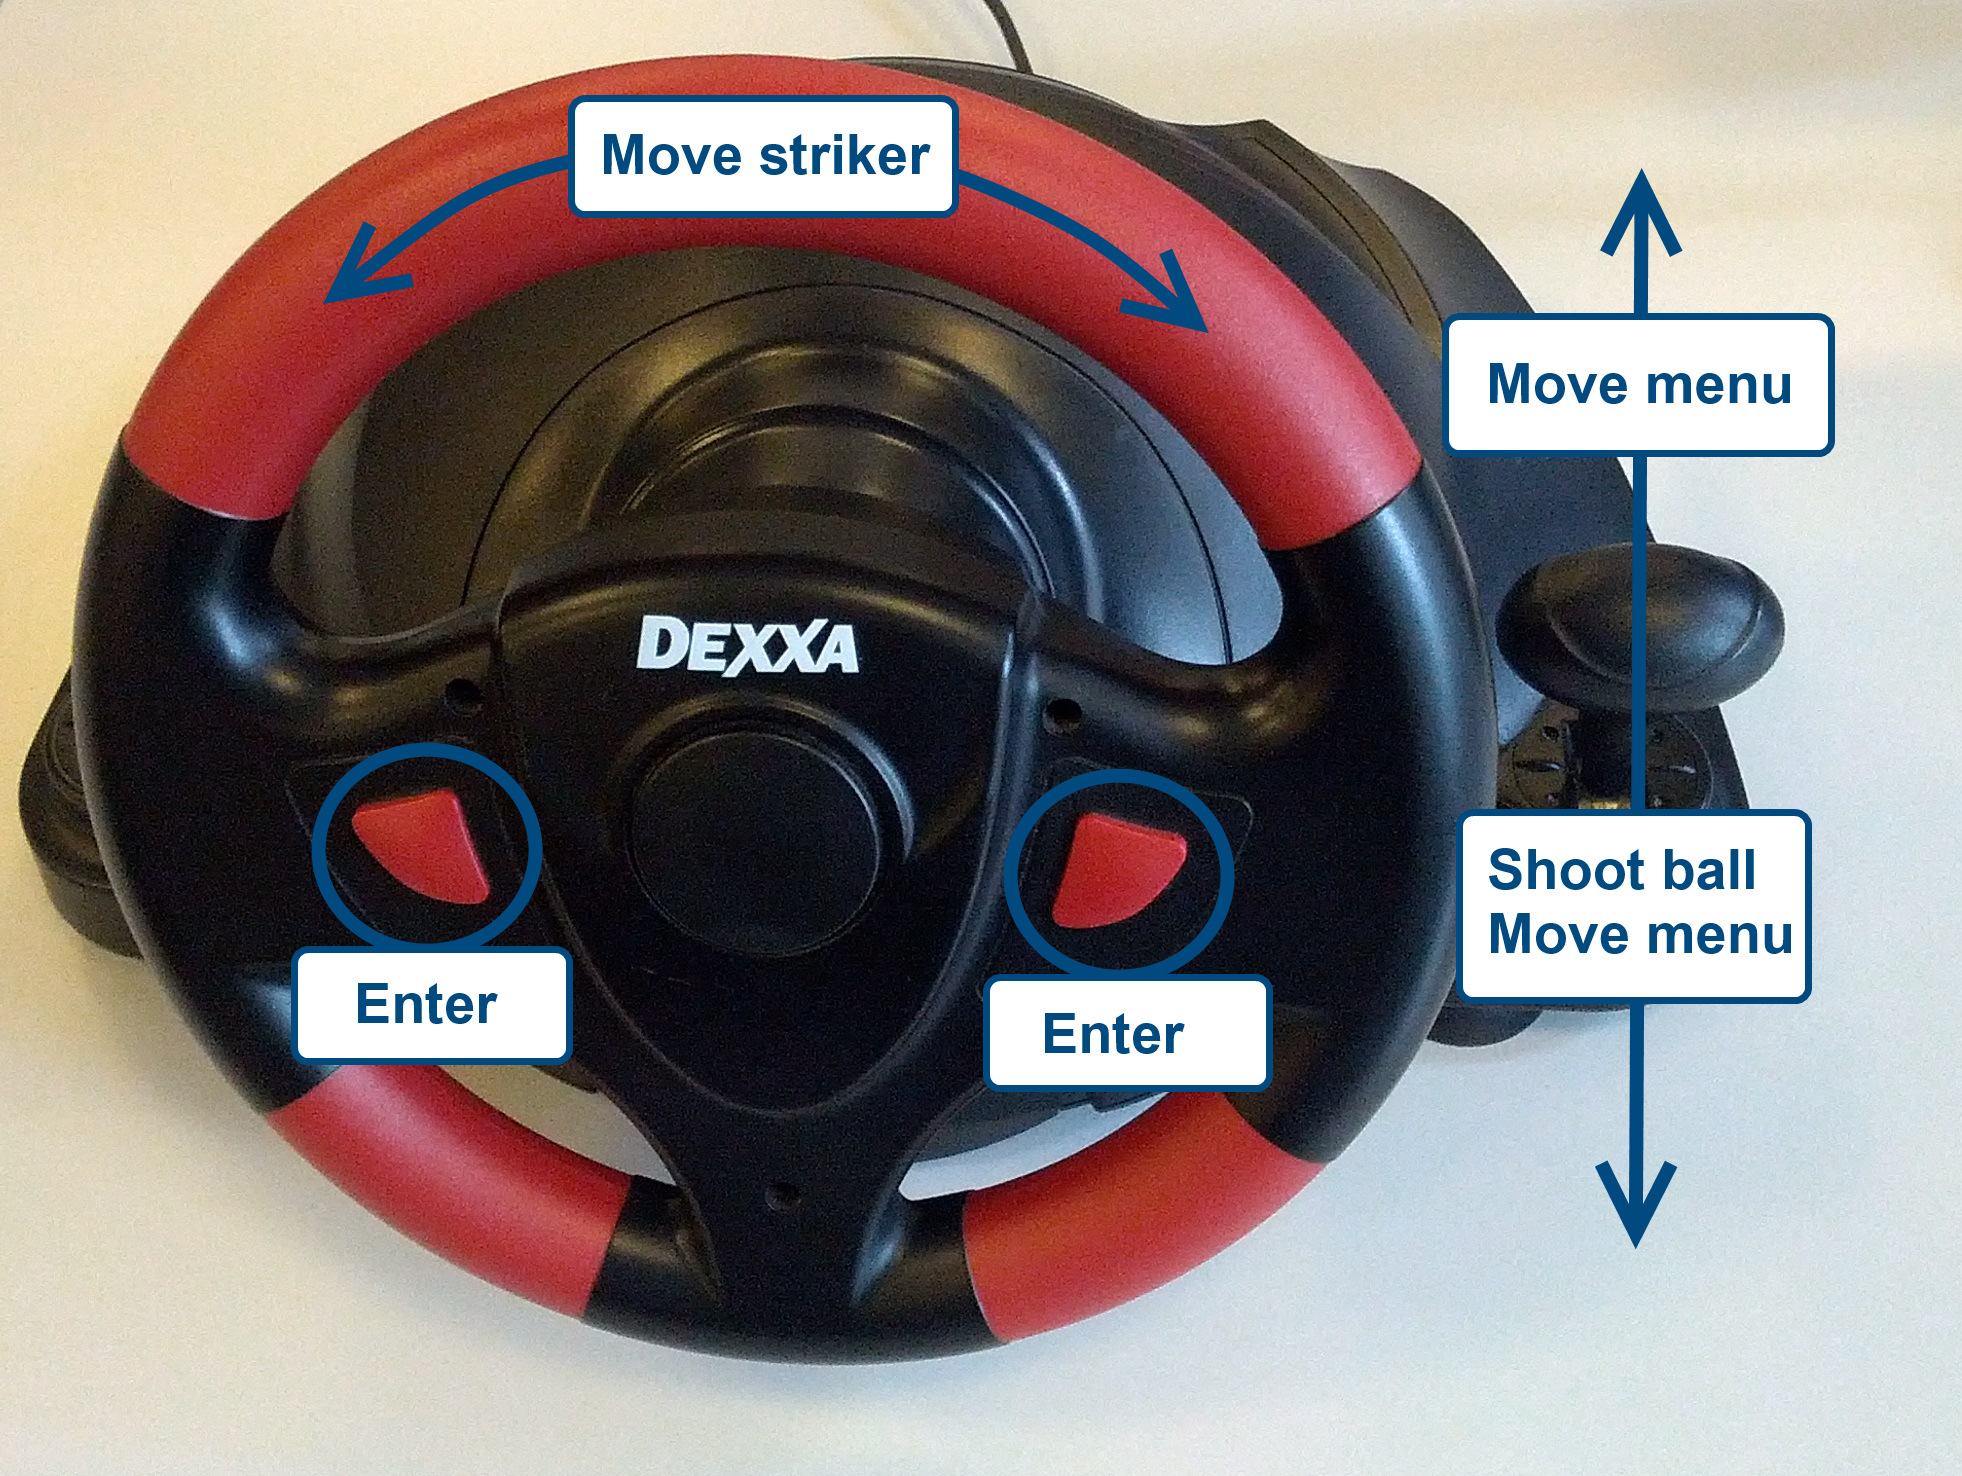
\includegraphics[width=\linewidth]{figs/rat_med_controls.png}
\caption{Oversigt over styring af rattet}
\label{fig:rat_med_controls}
\end{minipage}\hfill
\end{figure}

Derefter vises menuen svarende til den i figur \ref{fig:menu_2}. Her kan brugeren vælge sværhedsgraden. Brugeren kan således flytte bolden op og ned vha. gearet. Når den ønskede sværhedsgrad er valgt kan denne vælges ved at trykke på en af de to knapper der sidder på rattet. Den valgte sværhedsgrad bestemmer derefter bredden af strikeren, samt hvor hurtigt bolden skal begynde at forøge dens hastighed. Ved valg af Chuck Norris mode er boldens hastighed dog den maksimale hastighed fra starten. For mere information henvises til funktionen \nameref{asciidisplay} i appendiks \ref{C kode}. \\

\begin{figure}[h!]
\centering
\includegraphics[scale=0.25]{figs/screenshots/menu_crop.png}
\caption{Screenshot af menuen}
\label{fig:menu_2}
\end{figure}

Efter dette begynder selve spillet. Man skyder bolden afsted ved enten af at hive gearet tilbage eller trykke på en af de to knapper på rattet. Bolden vil da skydes afsted med en vinkel på 45-135 grader. Herefter gælder det blot om at skyde alle brikkerne ned ved at bevæge strikeren ved at dreje på rattet. Hvis brugeren skyder alle brikkerne i stykker avancerer brugeren til næste level. \\

Et overblik over alle de 6 levels i spillet kan ses på figurerne nedenfor. Bemærk at der i level 6 er en række usynlige brikker, der først kommer frem når man har ramt dem én gang. Se \nameref{levels} i appendiks \ref{C kode}. \\

\begin{figure}[h!]
\begin{minipage}[b]{0.32\textwidth}
\includegraphics[width=\linewidth]{figs/screenshots/level1.png}
\caption{Level 1}
\label{fig:level1_2}
\end{minipage}\hfill
\begin{minipage}[b]{0.32\textwidth}
\includegraphics[width=\linewidth]{figs/screenshots/level2.png}
\caption{Level 2}
\label{fig:level2}
\end{minipage}\hfill
\begin{minipage}[b]{0.32\textwidth}
\includegraphics[width=\linewidth]{figs/screenshots/level3.png}
\caption{Level 3}
\label{fig:level3}
\end{minipage}\hfill
\begin{minipage}[b]{0.32\textwidth}
\includegraphics[width=\linewidth]{figs/screenshots/level4.png}
\caption{Level 4}
\label{fig:level4}
\end{minipage}\hfill
\begin{minipage}[b]{0.32\textwidth}
\includegraphics[width=\linewidth]{figs/screenshots/level5.png}
\caption{Level 5}
\label{fig:level5}
\end{minipage}\hfill
\begin{minipage}[b]{0.32\textwidth}
\includegraphics[width=\linewidth]{figs/screenshots/level6.png}
\caption{Level 6}
\label{fig:level6}
\end{minipage}\hfill
\end{figure}

Hvis man taber spillet vises "Game Over!" skrevet med ASCII art, samt 1 tilfældig ud af 8 forskellige undertitler. Figur \ref{fig:gameover_2} viser et screenshot af dette. \\

\begin{figure}[h!]
\centering
\includegraphics[scale=0.25]{figs/screenshots/gameover_crop.png}
\caption{Eksempel på screenshot game over tekst}
\label{fig:gameover_2}
\end{figure}

Hvis man vinder spillet på Easy, Medium eller Hard vises et screenshot magen til figur \ref{fig:won_normal_2}, hvis man derimod vinder spillet på sværhedsgraden Chuck Norris vises et billedet som ses på figur \ref{fig:won_chuck}.

\begin{figure}[h!]
\begin{minipage}[b]{0.49\textwidth}
\includegraphics[width=\linewidth]{figs/screenshots/won_normal.png}
\caption{Screenshot ved gennemførsel af spillet}
\label{fig:won_normal_2}
\end{minipage}\hfill
\begin{minipage}[b]{0.49\textwidth}
\includegraphics[width=\linewidth]{figs/screenshots/won_chuck_crop.png}
\caption{Screenshot ved gennemførsel af spillet i Chuck Norris mode}
\label{fig:won_chuck}
\end{minipage}\hfill
\end{figure}
		\newpage
\chapter{Diskussion}
Bla bla. \\

Dette projekt valgte vi at dele op i en række delmål. Delmålene var delt op i grupperne Basics, Advanced, Brikker, Helhedsindtryk og Hardware. Basics var det der skulle til for at få et fungerende spil og de efterfølgende mål har skullet opfylde vores ønsker om at lave et realistisk spil med godt gameplay. Ud fra disse delmål, samt det ekstra mål at man skulle kunne få powerups i spillet, lavede vi tidsplanen vist på Figur \ref{fig:tidsplan2}, øverst. Som det kan ses nederst på samme figur, tog implementeringen af brikkerne dog væsentlig længere tid end forventet og det gjorde at vi ikke nåede vores mål om at lave powerups. Årsagen til dette var, at vi sammen med de avancerede delmål valgte at gøre bolden større. Da vi skiftede til terminalen putty i stedet for HyperTerminal og fik mulighed for at køre terminalen i fuldskærm valgte vi at lave bolden $4\times2$ karakterer. Dette gjorde at bolden kunne ramme flere brikker af gangen og briklogikken blev af den grund meget mere kompleks, se flowchartet på Figur \ref{fig:brickFlow} og  Appendix \nameref{reflexball} linje 145 og frem. En yderligere udfordring var at bolden bevægede sig to karakterer af gangen i x-retningen på skærmen. Der kunne derfor komme en stor del af bolden ind i brikkerne, hvilket også vanskeliggjorde at fastslå hvordan brikken var blevet ramt af bolden. \\ 
En stor del af arbejdet med brikkerne bestod derfor af debugging og rettelser i koden. For at teste briklogikken skrev vi tekst ud på skærmen der fortalte os hvordan vi havde ramt brikkerne, om flagene \texttt{dontDeflectX} og \dontDeflectY} var blevet sat og om det var detekteret at der var brikker ved siden af og over/under den ramte brik. På den måde kunne vi finde præcis de steder i koden hvor der var problemer med vores logik. 


Skriv verifikationsafsnit
	Globale variabler
	Problemer med brikker og bold
	Nåede ikke power-ups og power-downs
	Fandt undervejs ud af vi ville inkludere ASCII-Art
	Hvad vi nåede og hvad vi ikke nåede (se tidsplan2.png
	Hvordan vi har testet det hele


\begin{figure}[h!]
\centering
\includegraphics[scale=0.4]{figs/Tidsplan2.png}
\caption{Øverst: Tidsplan over de forskellige delmål og hvornår de skulle være færdige. Nederst: Hvad vi rent faktisk lavede og hvornår}
\label{fig:tidsplan2}
\end{figure}
		\newpage
\chapter{Konklusion}
Efter spillet et blevet designet, skrevet og uploadet til Zilog 6403 microcontrolleren, er alle spillets facetter blevet gennemtestet og fundet i overensstemmelse med det forventede resultat. Vi kan derfor konkludere at den skrevne kode implementerer spillet Reflex Ball på microcontrolleren og i hyperterminalen korrekt i forhold til specifikationskravene. Derudover kan vi også konkludere at alle udvidelse virker som forventet. \\


		\input{tex/Referencer}
		
	%%%	Appendix %%%		
		\newpage\appendix
		\chapter{Appendiks}
Henvis til: \url{https://github.com/Lauszus/ReflexBall}

%%%%%%%%%%%%%%%%%%%%%%%%
%%% THE BIBLIOGRAPHY %%%
%%%%%%%%%%%%%%%%%%%%%%%%

		
	
		
\end{document}
